\chapter{Batching Operations for Isogenies}

\section{Merging Signatures with \sidht}

\sidht and \sidh yeah

\begin{figure}[htp]
\centering
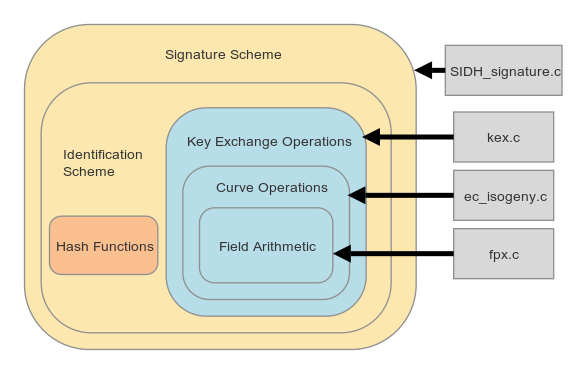
\includegraphics[scale=0.7]{fullmapwcurve.png} % e.g. insert ./image for image.png in the working directory, adjust scale as necessary
\caption{Relationship between SIDH based signatures \& Our fork of the SIDH C library}
\label{fig:fullmap} % insert suitable label, this is used to refer to a fig from within the text as shown above
\end{figure}

\section{Partial Batched Inversions}

One of our main contributions is the embedding of a low-level $\mathbb{F}_{p^{2}}$ procedure into Microsofts pre-existing SIDH library. The procedure in question reduces arbitrarily many unrelated/potentially parallel $\mathbb{F}_{p^{2}}$ inversions to a sequence of $\mathbb{F}_{p}$ multiplications \& additions, as well as one $\mathbb{F}_{p}$ inversion.\\

More specifically, the procedure takes us from \textit{n} $\mathbb{F}_{p^{2}}$  inversions to: 
\begin{center}
\begin{itemize}
\item 2\textit{n} $\mathbb{F}_{p}$ squarings
\item \textit{n} $\mathbb{F}_{p}$ additions
\item 1 $\mathbb{F}_{p}$ inversion
\item 3(\textit{n}-1) $\mathbb{F}_{p}$ multiplications
\item 2\textit{n} $\mathbb{F}_{p}$ multiplications
\end{itemize}
\end{center}


The procedure is as follows:\\

\begin{algorithm}
\caption{Batched Partial-Inversion}\label{euclid}
\begin{algorithmic}[1]
\Procedure{partial\_batched\_inv($\mathbb{F}_{p^{2}}$[ ] vec, $\mathbb{F}_{p^{2}}$[ ] dest, int n)}{}
\State initialize $\mathbb{F}_{p}$ $den[n]$
\For{\texttt{i = 0..(n-1)}}
	\State $den[i] \gets a[i][0]^{2} + a[i][1]^{2}$
\EndFor

\State $a[0] \gets den[0]$

\For{\texttt{i = 1..(n-1)}}
	\State $a[i] \gets \texttt{a[i-1]*den[i]}$
\EndFor

\State $a_{inv} \gets \texttt{inv(a[n-1])}$

\For{\texttt{i = n-1..1}}
	\State $a[i] \gets a_{inv}*dest[i-1]$
	\State $a_{inv} \gets a_{inv}*den[i]$
\EndFor

\State $dest[0] \gets a_{inv}$

\For{\texttt{i = 0..(n-1)}}
	\State $dest[i][0] \gets a[i]*vec[i][0]$
	\State $vec[i][1] \gets -1*vec[i][1]$
	\State $dest[i][1] \gets a[i]*vec[i][1]$
\EndFor
\EndProcedure
\end{algorithmic}
\end{algorithm}

\subsection{Projective Space}

Because the work of Yoo et al. was built on top of the original Microsoft SIDH library, all underlying field operations (and isogeny arithmetic) are performed in projective space. Doing field arithmitic in projective space allows us to avoid many inversion operations. The downside of this (for our work) is that the number opportunities for implementing the batched inversion algorithm becomes greatly limited.\\

\subsection{Remaining Opportunities}
There are two functions called in the isogeny signature system that perform a $\mathbb{F}_{p^{2}}$ inversion: j\_inv and inv\_4\_way. These functions are called once in SecretAgreement and KeyGeneration operations respectively. SecretAgreement and KeyGeneration are in turn called from each signing and verification thread.\\

This means that in the signing procedure there are 2 opportunities for implementing batched partial-inversion with a batch size of 248 elements. In the verify procedure, however, there are 3 opportunities for implementing batched inversion with a batch size of roughly ~124 elements.\\

\subsection{Constant Time vs. Binary GCD Inversion}

\section{Implementation Details}

\begin{figure}[htb]
\centering
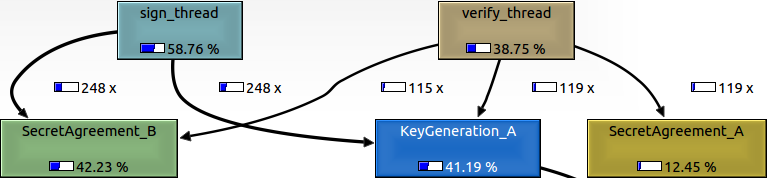
\includegraphics[scale=0.5]{signandverifycall} % e.g. insert ./image for image.png in the working directory, adjust scale as necessary
\caption{<Caption here>}
\label{fig:label} % insert suitable label, this is used to refer to a fig from within the text as shown above
\end{figure}

\section{Results}

Two different machines were used for benchmarking. System A denotes a single-core, 1.70 GHz Intel Celeron CPU. System B denotes a quad-core, 3.1 GHz AMD A8-7600.\\

The two figures below provide benchmarks for KeyGen, Sign, and Verify procedures with both batched partial inversion implemented (in the previously mentioned locations) and not implemented. All benchmarks are averages computed from 100 randomized sample runs. All results are measured in clock cycles.

\begin{center}
\begin{tabular}{@{}lllll@{}}
	\toprule
	Procedure & System A Without Batching & System A With Batching\\
	\midrule
	KeyGen & 68,881,331 & 68,881,331\\
	Signature Sign & 15,744,477,032 & 15,565,738,003\\
	Signature Verify & 11,183,112,648 & 10,800,158,871\\
	\bottomrule
\end{tabular}
\end{center}

\begin{center}
\begin{tabular}{@{}lllll@{}}
	\toprule
	Procedure & System B Without Batching & System B With Batching\\
	\midrule
	KeyGen & 84,499,270 & 84,499,270\\
	Signature Sign & 10,227,466,210 & 10,134,441,024\\
	Signature Verify & 7,268,804,442 & 7,106,663,106\\
	\bottomrule
\end{tabular}
\end{center}

\textbf{System A:} With inversion batching turned on we notice a ~1.1 \% performance increase for key signing and a ~3.5 \% performance increase for key verification.\\

\textbf{System B:} With inversion batching turned on we a observe a ~0.9 \% performance increase for key signing and a ~2.3 \% performance increase for key verification.\\

\subsection{Analysis}
It should first be noted that, because our benchmarks are measured in terms of clock cycles, the difference between our two system clock speeds should be essentially ineffective. \\

In the following table, "Batched Inversion" signifies running the batched partial-inversion procedure on 248 $\mathbb{F}_{p^{2}}$ elements. The procedure uses the binary GCD $\mathbb{F}_{p}$ inversion function which, unlike regular $\mathbb{F}_{p^{2}}$ montgomery inversion, is not constant time.\\

\begin{center}
\begin{tabular}{@{}ll@{}}
	\toprule
	Procedure & Performance \\
	\midrule
	Batched Inversion & 1721718\\
	$\mathbb{F}_{p^{2}}$ Montgomery Inversion & 874178\\
	\bottomrule
\end{tabular}
\end{center}

Do performance increases observed make sense?\\

